% $Header: /cvsroot/latex-beamer/latex-beamer/examples/beamerexample3.tex,v 1.8 2004/10/07 20:53:07 tantau Exp $

\documentclass{beamer}
% Usar linha abaixo caso queira gerar uma versao para impressao
%\documentclass[handout]{beamer}
%\usepackage{handoutWithNotes}

%\pgfpagesuselayout{4 on 1 with notes}[a4paper,border shrink=5mm]

%\usetheme{Warsaw}
%\usetheme{Dresden}
%\usetheme{Berlin}
%\usetheme{Hannover}
%\usetheme{Berkeley}
%\usetheme{CambridgeUS}
\usetheme{progressbar}
%\usecolortheme{crane}

\usepackage[english]{babel}
\usepackage[latin1]{inputenc}
\usepackage{graphicx}
\usepackage{amsmath,amssymb}
%\usepackage{algorithm}                             % when including figure files
\usepackage{sansmathaccent}
\pdfmapfile{+sansmathaccent.map}
\usepackage{epstopdf}
\usepackage{epsfig}

\setbeamercovered{transparent}
\newtheorem{rem}{Remark}
\newtheorem{proposition}[theorem]{Proposition}
\newtheorem{step}{Step}

%\newtheorem{example}[theorem]{Example}

\title{IBM Research Seminar}
\author{Carlos Raoni de Alencar Mendes}
\institute{Software Engineer - Petrobras \\
\texttt{carlosraoni@gmail.com} }

\begin{document}


\frame{\titlepage}

\begin{frame}
	\scriptsize
  \tableofcontents[pausesections]
\end{frame}

\section{Resume}
\subsection{Education}

\begin{frame}
  \frametitle{Education}
{
	\begin{itemize}
		\item<1-> {\bf Ph.D.}, Computer Science, Pontifical Catholic University of Rio
		de Janeiro (PUC-RJ), 2012 - Present.			
  		\item<2-> {\bf M.Sc.}, Computer Science, Pontifical Catholic University of
  		Rio de Janeiro (PUC-RJ), 2007 - 2009.
  			\begin{itemize}
			  \item GPA (ranging from 0 to 10): 9.6
			  \item Classes on Algorithm Analysis, Machine Learning, Combinatorial
			  Optimization, Linear Programming, Information Retrieval and Search Engines, among others.
			  \item I was the only Computer Science master student of PUC-RJ to publish in 2009 a paper in a high 
qualified international journal according to criteria of Brazilian foundation
for supporting academic research (CAPES).
			\end{itemize}
  		\item<3-> {\bf B.Sc.}, Computer Science, Federal University of Rio Grande do
  		Norte (UFRN), 2002 - 2006.
  			\begin{itemize}
			  \item GPA (ranging from 0 to 10): 9.132
			  \item Second best GPA
			\end{itemize}
  \end{itemize}
}

\end{frame}

\subsection{Research scholarship (UFRN), 2004 - 2006}

\begin{frame}
	\frametitle{Research scholarship (UFRN), 2004 - 2006}
{
	
	  \begin{itemize}
	    \item<1-> Development of a new evolutionary multi-objective algorithm
	    for optimization of treatment planning of conformal radiation therapy.
		\begin{figure}[ht]
			\begin{minipage}[b]{0.45\linewidth}
				\centering
				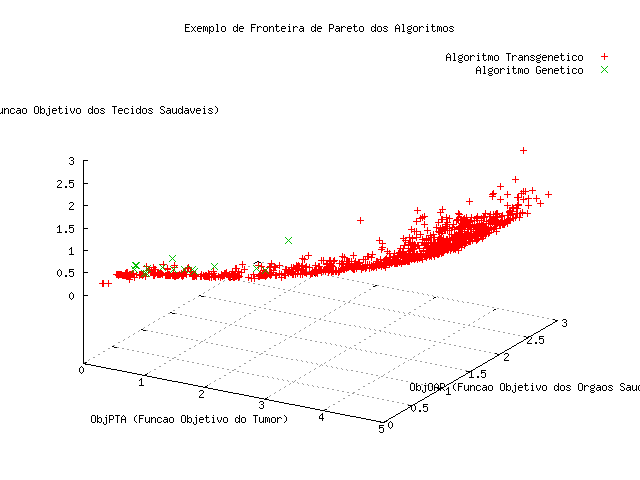
\includegraphics[width=0.80\textwidth]{images/front.png}
				\label{fig:pareto}				
			\end{minipage}
			\hspace{0.5cm}
			\begin{minipage}[b]{0.45\linewidth}
				\centering
				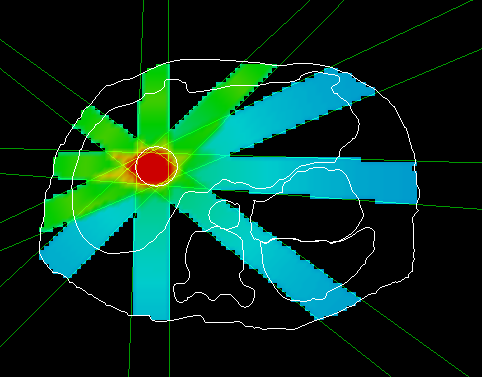
\includegraphics[width=0.80\textwidth]{images/trans1.PNG}
				\label{fig:transsolution}				
			\end{minipage}
		\end{figure}
		\begin{itemize}
			\item<2-> Published paper in Brazilian journal \textbf{Pesquisa
			Operacional (Operations Research)}: \textit{Evolutionary algorithm to
			optimize the treatment plan in 3D conformal radiotherapy}, 2009.
			\item<3-> Published extended abstract in proceedings of the international
			conference \textbf{23rd Annual ACM Symposium on Applied Computing}:
			\textit{Selecting beam directions in radiotherapy with an evolutionary algorithm}, 2008.  
		\end{itemize}
		
	  \end{itemize}	  		
}
\end{frame}

\subsection{Research scholarship (PUC-Rio), 2007 - 2009}

\begin{frame}
	\frametitle{Research scholarship (PUC-Rio), 2007 - 2009}
{
	\begin{itemize}
	  \item<1-> Member of the development and research team of PRONAV project.
	  \item<2-> Optimization module to assist the programming of ships routes (and
	  operations) in order to take care of the products transport demands of
	  Petrobras.	  
	  \item<3-> Main technologies: C++ and CPLEX solver.
	  \item<4-> Multi-Commodity Network Flow based MIPs.	  	    	  
	\end{itemize}
}
\end{frame}

\begin{frame}
	\frametitle{Research scholarship (PUC-Rio), 2007 - 2009}
{
	\begin{figure}[htbp]			
		\centering
		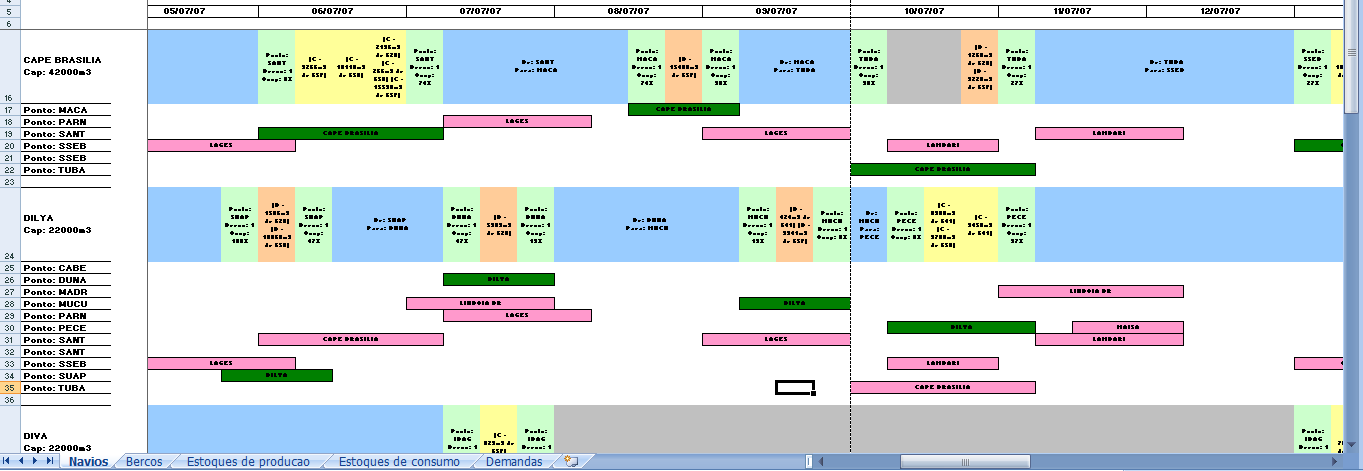
\includegraphics[width=0.60\textwidth]{images/navios.png}
		\label{fig:navios}
		\caption{\small{Ships Routes}}							
	\end{figure}	
	\begin{figure}[htbp]			
		\centering
		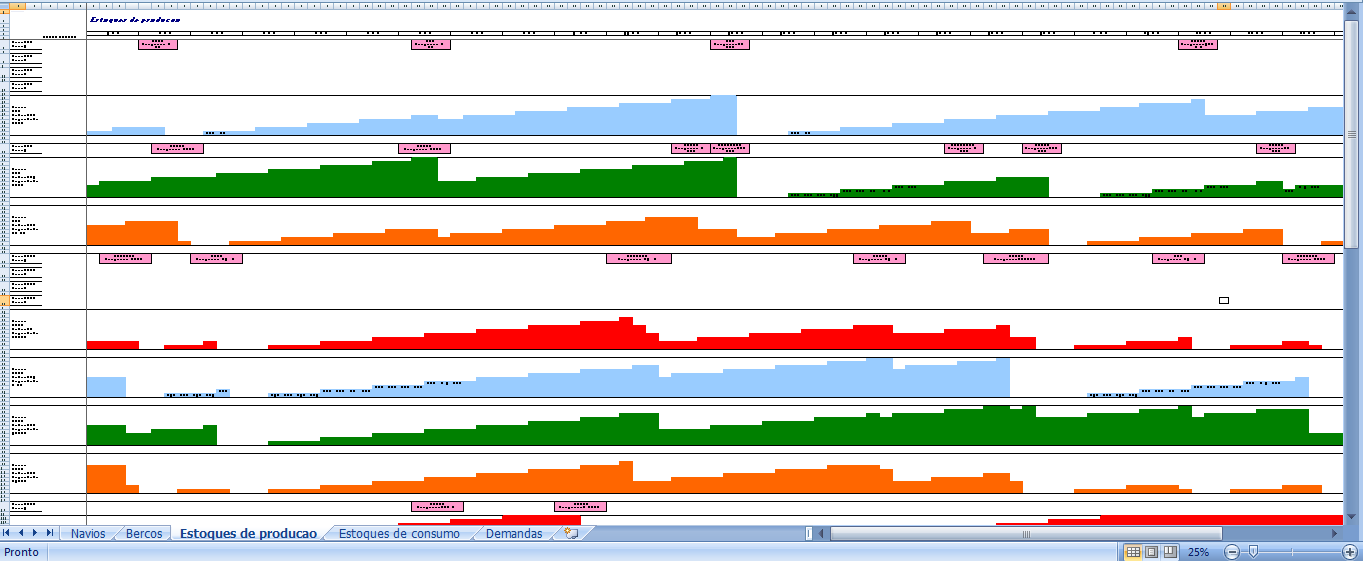
\includegraphics[width=0.60\textwidth]{images/estoques.png}
		\label{fig:estoques}
		\caption{\small{Oil Platforms Storage}}							
	\end{figure}
}
\end{frame}

\begin{frame}
	\frametitle{Research scholarship (PUC-Rio), 2007 - 2009}
{
	\begin{itemize}
	  \item<1-> Development of heuristic algorithms for covering codes problems.
	  \item<2-> Master's Thesis Research Theme.  
	  \item<3-> Published paper in the international journal \textbf{Discrete
	  Applied Mathematics}: \textit{Bounds for short covering codes and reactive tabu search}, 2009.	  
	  \item<4-> Published paper in proceedings of \textbf{XXXIX Brazilian
	  Symposium of Operational Research}: \textit{Upper Bounds for Minimum Short 
Covering Codes by Reactive Tabu Search}, 2007.	  	    	  
	\end{itemize}
}
\end{frame}

\subsection{Software Engineer(Petrobras), 2008 - Present}

\begin{frame}
	\frametitle{Software Engineer(Petrobras), 2008 - Present}
{
	\begin{itemize}
	  \item<1->Object-oriented architecture, design and development of Desktop and
	  Web-Based enterprise systems.
	  \item<2->Main technologies: Java EE (EJB 3, JMS, Web Services), C\# .Net,
	  Oracle Database and others.
	  \item<3->Past project: a torque calculation system for screws of bolted
	  joints. Software developed in C\# .Net.
	\end{itemize}		 
}
\end{frame}

\begin{frame}
	\frametitle{Software Engineer (Petrobras), 2008 - Present}
{	 
	\begin{figure}[htbp]			
		\centering
		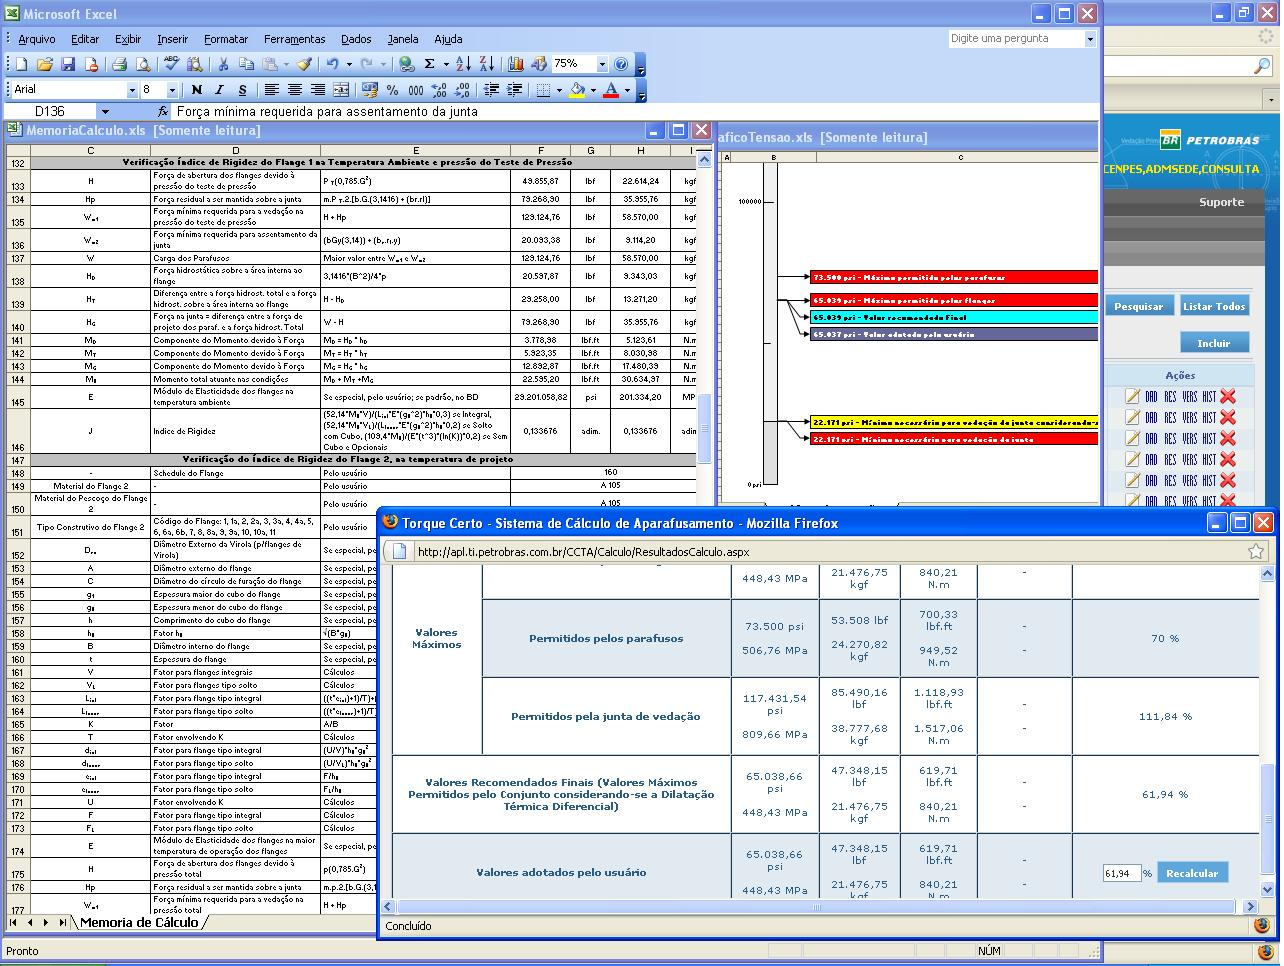
\includegraphics[width=0.70\textwidth]{images/ccta.JPG}
		\label{fig:ccta}
		\caption{\small{Business Value Maximization Award of Systems Development
		Department of Information Technology and Communications (ITC) Division, 2010}}							
	\end{figure}
}
\end{frame}

\begin{frame}
	\frametitle{Software Engineer (Petrobras), 2008 - Present}
{
	\begin{itemize}
	  \item<1->Current project: an enterprise system to control fluid transfers operations in refinery plants, in order to transform crude oil into more useful petroleum 
products, such as gasoline, diesel fuel and kerosene. 
	  \item<2->Java swing client that shows and controls the status of the fluid
	  transfers, refinery equipments, commands to equipments, and so on. 
	  \item<3->The client interacts with the back-end system developed in EJB 3:
	  	\begin{itemize}
	  	  \item JMS Topics and Queues
	  	  \item XA Transactions
	  	  \item Web Services, and so on
	  	\end{itemize}
	 \item<4-> Integration with a planning system through EJB technology and with
	 an automation system through a CORBA interface.
	 \item<5-> Individual Distinction Award of the ITC division for the outstanding
	 work performance in 2011.
	\end{itemize}		 
}
\end{frame}

\subsection{Problem Solving Competitions}

\begin{frame}
	\frametitle{Problem Solving Competitions}
{
	\begin{itemize}
	  \item<1->Algorithm analysis and programming competitions.
	  \item<2->\textbf{ACM International Collegiate Programming Contest} - Brazil:
	  Four times Brazilian finalist, from 2004 to 2007.
	  \item<3->\textbf{Google Code Jam Latin America 2007}: Advancer of
	  Qualification Round and Online Round 1, finishing in Top 70 in semifinals.
	  \item<4->\textbf{ACM UVA Problem Solving Website}: As an undergrad I was in
	  the Brazilian Top 30 and World Top 500 at the ACM UVA (acm.uva.es) problem solvers ranking with 305 solved problems.
	  \item<5->\textbf{ProjectEuler.net Website}: Top 30 of the ProjectEuler.net
	  Brazilian ranking with 101 solved problems.
	\end{itemize}		 
}
\end{frame}

\section{Covering Codes}

\begin{frame}
  \frametitle{Covering Codes: Bounds and Heuristics}
{	
\begin{itemize}
	\item<1-> Data compression, speech coding, mobile telecommunications and error-correction are some of the practical applications of the covering codes study.
	\item<2-> This work addresses two problems of covering codes: 
	\begin{enumerate}
		\item<3-> The classic code covering problem
		\item<4-> And the recent variant called short code covering problem
	\end{enumerate}
	\item<5-> It presents an application of Reactive Tabu Search (RTS) metaheuristic for this problems.
	\item<6-> It also presents a new heuristic technique that combines the delayed column generation and local search heuristics, the so called Column Generation Improvement Heuristic (CGIH).
\end{itemize}
}
\end{frame}


\begin{frame}
  \frametitle{The Football Pool problem}
{
	
\begin{itemize}
	\item<1-> An interesting application of covering codes is trying to win at football pools.
	\item<2-> Filling and submitting a football pool ticket is to give forecasts for the outcome of a given number football matches.
	\item<3-> Each football match has three possible outcomes: home win `1', draw `x' or away win `2'.
	\item<4-> The football pool problem: How many tickets are to be submitted to guarantee the second prize (miss at most one match)?
	\item<5-> The case where we have 6 matches has been object of a tremendous effort in improving the best known lower bound to 71, while its upper bound remains at 73.
\end{itemize}
}
\end{frame}

\subsection{Coding Theory Definitions}

\begin{frame}
  \frametitle{Coding Theory Definitions}
{
	
\begin{itemize}
	\item<1-> We call alphabet $\Bbb{F}_{q}$ the set of $q$ symbols $\Bbb{F}_{q} = \{0, 1, ..., q-1\}$.
	\item<2-> When $q$ is a prime power is convenient consider $\Bbb{F}_{q}$ as a finite field with $q$ elements.
	\item<3-> A word is a $n$-dimensional vector with symbols of $\Bbb{F}_{q}$.
	\item<4-> $\Bbb{F}_{q}^{n}$ is the set of all words of size $n$ over $\Bbb{F}_{q}$.
	\item<5-> A q-ary code is a non-empty subset of $\Bbb{F}_{q}^{n}$.
\end{itemize}
}
\end{frame}


\begin{frame}
  \frametitle{Coding Theory Definitions}
{
	Examples with $n=3$ and $q=2$:
\begin{itemize}
	\item Alphabet: $\Bbb{F}_{2} = \{0,1\}$.
	\item Word: $x = (001)$.
	\item Words Space: $\Bbb{F}_{2}^{3} = \{(000), (001), (010), (011), (100),$ $ (101), (110), (111)\}$.
	\item q-ary code of $\Bbb{F}_{2}^{3}$: $C = \{(001), (110), (100)\}$.
\end{itemize}

\begin{block}{Definition}[\textit{Hamming Distance}]
The Hamming distance $d(x,y)$ between two words $x = (x_1 \ldots x_n)$ and $y = (y_1 \ldots y_n)$ is the number of components in which x and y differ (i.e., $|{x_i \neq y_i, 1 \leq i \leq n}|$).
\end{block}

}
\end{frame}


\begin{frame}
  \frametitle{Coding Theory Definitions}
{

\begin{block}{Definition}[\textit{Hamming Sphere}]
\textit{Hamming Sphere} is the sphere of center $x$ and radius $R$ denoted by: 
\begin{equation}
\label{esfera}
B(x,R)=\{y \in F_{q}^{n}:\,\,d(x,y)\leq R\}.
\end{equation}
\end{block}

\begin{figure}[htbp]
	\centering
		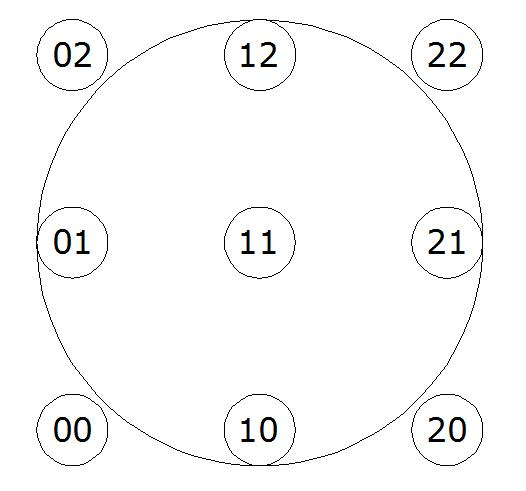
\includegraphics[width=0.30\textwidth]{images/boundingsphere.jpg}
	\label{fig:bouding}
	\caption{\textsl{Hamming Sphere} with center $x = (11)$, $R=1$ over $\Bbb{F}_{3}^{2}$.}
\end{figure}

}
\end{frame}

\subsection{Covering Codes and Short Covering Codes}

\begin{frame}
  \frametitle{The Classic Covering Codes Problem}
{
	
\begin{itemize}
	\item<1-> Given integers $q\geq 2$, $n\geq 1$ and $R\geq 0,$ we denote $K_{q}(n,R)$ as the minimum cardinality of a set of codewords $C$ in any $q$-ary code of length $n$ such that for every word $x$, there is a codeword $c$ in $C$ in which $x$ and $c$ disagree in at most $R$ coordinates.
	\item<2-> The determination of $K_{q}(n,R)$ for any $n$, $q$ and $R$ is the classical covering codes problem.
	
\begin{block}{Definition}[$K_{q}(n,R)$]
{
\scriptsize
	For $n\geq 2$ and $q\geq 2$, let $V_{q}^{n}$ be the set of all words $x$ = ($% 
x_{1}x_{2}\ldots x_{n}$) with length $n$ and components $x_{i}$
taken on any alphabet of $q$ symbols. A subset $C$ is an $R$-\textit{covering} of $V_{q}^{n}$ when:
\[
\bigcup_{c\in C}B(c,R)=V_{q}^{n}.
\]
Thus, the number $K_{q}(n,R)$ denotes the minimum cardinality of an $R$-%
{\it covering} of $V_{q}^{n}.$

}
\end{block}
	
\end{itemize}
}
\end{frame}


\begin{frame}
  \frametitle{Short Covering Codes Problem}
{
	
\begin{itemize}
	\item<1-> Let $\Bbb{F}_{q}$ denote the finite field with $q$ elements. Given integers $n\geq 2$ and $0 \leq R \leq n$, define $c_{q}(n,R)$ as the minimum cardinality of a subset $H$ of $\Bbb{F}_{q}^{n}$ such that every word $x$ in this space differs in at most $R$ coordinates from a scalar multiple of a vector in $H$.
	\item<2-> The determination of $c_{q}(n,R)$ for any $q$, $n$ and $R$ is the short covering codes problem.
\end{itemize}	 

}
\end{frame}


\begin{frame}
  \frametitle{Short Covering Codes Problem}
{
	
\begin{block}{Definition}[$R$-\textit{short covering}]
\scriptsize
	A subset $H$ in the vector space $\Bbb F_{q}^{n}$ is an $R$-\textit{short covering\ of }$
\Bbb F_{q}^{n}$ when $ \Bbb F_{q}.H=\{\alpha h,\alpha \in \Bbb F_{q} \mbox{ and } h\in H\}$ is an $R$%
-covering of $\Bbb F_{q}^{n}$.
\end{block}
\pause

\begin{itemize}
	\item It is worth stating that $H$ is a short covering iff the set that contains $H$ and all their scalar multiples generates a covering of $\Bbb F_{q}^{n}$.
\end{itemize}

\begin{block}{Definition}[$c_{q}(n,R)$]
\scriptsize
The induced extremal problem $c_{q}(n,R)$ is defined as the minimum cardinality of such subset $H$, i.e:
\[
c_{q}(n,R)=\min \{\ \left| H\right| :H \mbox{ is an } R
\mbox{-short covering of } \Bbb F_{q}^{n}\mathit{\ }\}.
\]\end{block}

}
\end{frame}


\begin{frame}
  \frametitle{Motivations for Studying Short Covering Codes}
{
\begin{itemize}

\item<1-> On the basis of theoretical viewpoint, short covering seems to be an algebraic structure richer than classical covering, since short covering is invariant under scalar multiplication. 
\item<2-> From a practicable point of view, short coverings provide us with a way to store codes using less memory than the classical ones.
\item<3-> Results on short covering codes may bring us record-breaking results on classical codes.

\end{itemize}

}
\end{frame}

\subsection{Covering Codes and Dominating Sets in Graphs}

\begin{frame}
  \frametitle{Dominating Sets in Graphs}
{


\begin{block}{Definition}[Dominating Set]
\scriptsize
Let $G=(V,E)$ be a directed graph with node set $V$ and a collection $E$ of ordered pairs in $V\times V$. 
As usual, $u$ is adjacent to $v$ (or $v$ is a neighbor from $u$) when $(u,v) \in E$. The node set $U \subseteq V$
is said to be a {\it dominating set} of $G$ if, for every node $v$ in $V$, either $v$ is in $U$ or there exists a node $u$ in $U$ such that $u$ is adjacent to $v$ ({\em i.e.}, $(u,v) \in E$).
\end{block}
\pause

\begin{itemize}
\item<1-> The dominating set problem is the problem of finding a dominating set in the graph (or digraph) whose size is minimum. 
\item<2-> Both covering codes problems described correspond to a class of the dominating set problem in digraphs.
\end{itemize}

}
\end{frame}


\begin{frame}
  \frametitle{Covering Codes and Dominating Sets in Graphs}
{

\begin{itemize}

\item<1-> Given the vector space $\Bbb{F}_q^n$ and $0 \leq R \leq n$, let us construct the digraph $G(n,q,R)=(V,E)$.
\item<2-> For each vector $u$ in $\Bbb{F}_q^n$ we associate a node $u$ in $V$.
\item<3-> The edge $e=(u,v)$ is in $E$ if and only:
 	\begin{itemize}
 	  \item<4-> $d(u,v) \leq R$ for the classical covering codes problem
 	  \item<5-> there is $\alpha \in \Bbb{F}_q$ such that $0 <d(\alpha u,v) \leq R$ for the short covering codes problem
	\end{itemize}
\item<6-> Note that we can solve both covering codes problems by solving the minimum dominating set problem in $G(n,q,R)$.

\end{itemize}

}
\end{frame}


\begin{frame}
  \frametitle{Covering Codes and Dominating Sets in Graphs}
{

\begin{figure}
	\centering
		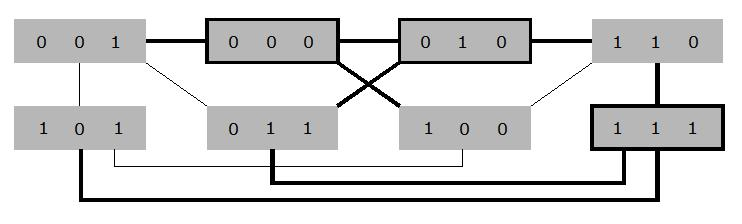
\includegraphics[width=7cm]{images/s3.jpg}
	\label{fig:solucao}
	\caption{\footnotesize Dominating Set for $K_{2}(3,1)$.}
\end{figure}

\begin{figure}
	\centering
		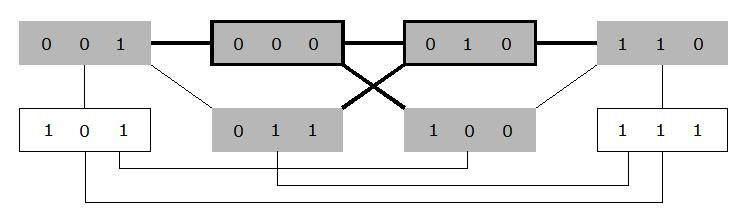
\includegraphics[width=7cm]{images/s2.jpg}
	\label{fig:solucaoinviavel}
	\caption{\footnotesize Unfeasible solution for $K_{2}(3,1)$.}
\end{figure}

}
\end{frame}


\begin{frame}
  \frametitle{Covering Codes and Dominating Sets in Graphs}
{


\begin{figure}
	\centering
		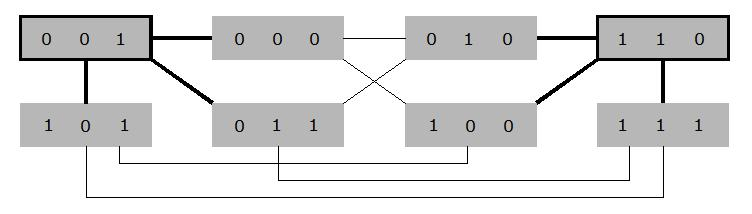
\includegraphics[width=7cm]{images/s1.jpg}
	\label{fig:solucaootima}
	\caption{\footnotesize Optimal solution for $K_{2}(3,1)$.}
\end{figure}

}
\end{frame}

\subsection{Related Work}

\begin{frame}
  \frametitle{Related Work}
{
	
\begin{itemize}
  	\item<1-> Local search has been successfully used in many papers to construct
  	good covering codes.
	\item<2-> Early works utilized almost exclusively \textsl{Simulated Annealing}.
		\begin{enumerate}
			\item Wille 1987 - $K_{3}(6,1) \leq 74$.
			\item Van Laarhoven et al. 1989- $K_{3}(6,1) \leq 73$ e $K_{3}(7,1) \leq
		186$.
		\end{enumerate}
	\item<3-> \"Osterg\aa rd 1991, Wille 1990, Aarts et. al 1992 e Van Lint 1989
	also achieved a large number of record breaking results using \textsl{Simulated
	Annealing}.
	\item<4-> \"Osterg\aa rd 1997 was the first work using Tabu Search on covering
	codes.
	\item<5-> W.A. Carnielli et. al 1998 used a different search space and also applied tabu search on covering codes.	
\end{itemize}
}

\end{frame}

\section{Reactive Tabu Search}

\begin{frame}
  \frametitle{Reactive Tabu Search on Covering Codes Problems}
{
	
\begin{itemize}
  	\item<1-> Carnielli at al. and \"Osterg\aa rd use metaheuristics to find upper bounds for $R$-covering codes. Neither of these works used the reactive variation of Tabu Search.	
	\item<2-> Tabu Search (TS) is an adaptive local search procedure.
	\item<3-> The main goal of TS is to avoid the existence of cycles in the search path while inducing a broad search of the solution space as well as an intensive search on promising regions.	
	\item<4-> The neighborhood moving is almost always a greedy step. However, we can only move from the current solution to one of the solutions in its neighborhood when the corresponding movement is not ``Tabu'' marked.	
	\item<5-> The classical TS scheme keeps a list (tabu list) of fixed size, this allows cycles larger than the list size.			
\end{itemize}
}
\end{frame}

\begin{frame}
  \frametitle{Reactive Tabu Search on Covering Codes Problems}
{
	
\begin{itemize}
    \item<1-> Battiti and Tecchiolli proposed a reaction mechanism to help tabu search to overcome local minimum traps, creating the Reactive Tabu Search (RTS).
    \item<2-> It amounts to combine the main elements of a TS with a long term memory of the search that keeps a history of the visited solutions.	
	\item<3-> This memory is used to dynamically control the size of the tabu list, augmenting its size when cycling becomes frequent and reducing it when a new region starts to be explored. 	
	\item<4-> RTS also has a local minimum scape mechanism via successive random perturbations.	
	\item<5-> RTS has had a reasonable success in several applications.
\end{itemize}
}
\end{frame}

\subsection{The Basic Tabu Search Scheme}

\begin{frame}
  \frametitle{The Basic Tabu Search Scheme}
{
	
\begin{itemize}
	\item<1-> Search Space: the set of all $2^{(q^n)}$ subsets of $\Bbb{F}_q^n$ (the vertex set of $G(n,q,R)$).
	\item<2-> Neighborhood: adding a vertex not in the current solution set or removing one vertex from this set.
	\item<3-> Objective Function: the size of the dominating set added with a penalty factor.
	\item<4-> Tabu List: store the number of the last iteration where a movement (a vertex switch) was made tabu.
	\item<5-> Aspiration Criteria: a solution can violate the tabu restriction when it improves the value of the best solution found until this point in the search.
\end{itemize}
}
\end{frame}


\begin{frame}
  \frametitle{The Basic Tabu Search Scheme}
{
{\bf Initializations.}
\begin{itemize}
    \item[-] Construct an initial Cover $U$ by adding random selected words, not in $U$, until $U$ is a Cover.
    \item[-] $BestCode \leftarrow U$.
    \item[-] $T[M] \leftarrow 0$, for every possible move $M$.
    \item[-] $alpha \leftarrow MIN\_ALPHA$.
    \item[-] Initialize Reaction Mechanism.
\end{itemize}	
}
\end{frame}


\begin{frame}
  \frametitle{The Basic Tabu Search Scheme}
{
{\bf Main Loop.} Repeat {\sc Number-of-Iterations} times.
\begin{itemize}
    \item[-] Update Penalty Factor ($alpha$).
    \item[-] Select the best move $M$ that is not tabu or satisfies the aspiration criteria.
    \item[-] Make a Move $M$ in $U$.
    \item[-] Set a tabuValue of $M$ in $T$, $T[M]  \leftarrow current-iteration$.
    \item[-] \textbf{If} $U$ is a cover and $|U| < |BestCode|$
        \begin{itemize}
        \item[-] $BestCode \leftarrow U$.
        \end{itemize}
    \item[-] {\bf Call Reaction Mechanism}.
\end{itemize}
}
\end{frame}

\subsection{The Reaction Mechanism}

\begin{frame}
  \frametitle{Dynamic Tabu Tenure Control and Scape Mechanism}
{
	
\begin{itemize}
	\item<1-> Long term memory keeping track of the solutions visited, the iteration when they were last visited and how many times they became a current solution.
	\item<2-> Each time a solution repeats in the search the interval between visits is calculated.
	\item<3-> A quick reaction occurs when this interval is smaller than a given threshold, this reaction is to set the tabu tenure to a large value.
	\item<4-> A slow reaction follows gradually reducing the tabu tenure. 
	\item<5-> The scape mechanism: keeping track of the solutions that are visited an excessive number of times, when this number of solutions goes beyond a given threshold, a number of random moves is done on the current solution.
	
\end{itemize}
}
\end{frame}


\begin{frame}
  \frametitle{The Reaction Mechanism Algorithm}
{
	
{\bf Reaction Mechanism Initialization}
\begin{itemize}
    \item[-] Create empty sets $Visited$ and $OftenReapeated$.
    \item[-] $chaotic \leftarrow 0$.
    \item[-] $countLastSizeChange \leftarrow 0$.
    \item[-] $movingAvg\leftarrow 0$.
    \item[-] $tabuTenure \leftarrow MIN\_TENURE$.
\end{itemize}
}
\end{frame}

\begin{frame}
  \frametitle{The Reaction Mechanism Algorithm}
{
{\bf Reaction Mechanism}

\begin{itemize}
\item[-] $escape \leftarrow true$. \item[-]
$countLastSizeChange++$. \item[-] \textbf{If} $U$ is in $Visited$.
    \begin{itemize}
    \item[-] $TamCycle \leftarrow$ current iteration - last visit iteration of $U$.
    \item[-] Increment the number of visits of $U$ and update the iteration of last visit to $U$.
    \item[-] \textbf{If} $TamCycle < CYCLE\_MIN$.
        \begin{itemize}
        \item[-] $movingAvg \leftarrow 0.9 * movingAvg + 0.1 * TamCycle$.
        \item[-] $tabuTenure \leftarrow min(tabuTenure * INCREASE, MAX\_TENURE)$.
        \item[-] $countLastSizeChange \leftarrow 0$.
        \end{itemize}
    \item[-] \textbf{If} number of visits to $U > MAX\_VISITS$ and $U$ is not in $OftenRepeated$
        \begin{itemize}
        \item[-] Insert $U$ in $OftenRepeated$ and increment $chaotic$.
        \item[-] \textbf{If} $chaotic > Chaos$: $escape \leftarrow true$.
        \end{itemize}
    \end{itemize}
\end{itemize}

}

\end{frame}


\begin{frame}
  \frametitle{The Reaction Mechanism Algorithm}
{
{\bf Reaction Mechanism}

\begin{itemize}
\item[-] \textbf{Else}
    \begin{itemize}
    \item[-] Insert $U$ in $Visited$ and set the number of visits to $U$ to one and the last iteration of a visit to $U$ to the current iteration.
    \item[-] \textbf{If} $countLastSizeChange > movingAvg$.
        \begin{itemize}
        \item[-] $tabuTenure \leftarrow max(tabuTenure * DECREASE, MIN\_TENURE)$.
        \item[-] $countLastSizeChange \leftarrow 0$.
        \end{itemize}
    \end{itemize}
\item[-] \textbf{If} $escape$ is $true$.
    \begin{itemize}
    \item[-] Clear the $Visited$ set.
    \item[-] $chaotic \leftarrow 0$.
    \item[-] Make a random number of moves in $U$.
    \end{itemize}
\end{itemize}
}

\end{frame}


\section{CGIH}

\begin{frame}
  \frametitle{Column Generation Improvement Heuristic (CGIH)}
{
	
\begin{itemize}
	\item<1-> The CGIH is a new heuristic technique that combines a search space transformation based on delayed column generation and local search procedures.
	\item<2-> The search space transformation is used to help the local search to escape from local minimums.
	\item<3-> This transformation is based on the pricing problem from the delayed column generation model.
	\item<4-> The basic strategy is to apply the search space transformation and then restart the search in this new space.
	
\end{itemize}
}
\end{frame}


\subsection{Search Space Transformation}

\begin{frame}
  \frametitle{Search Space Transformation}
{
	
\begin{itemize}
	\item<1-> When:
		\begin{itemize}
		 	\item<2-> the columns of the column generation formulation are viable solutions to the problem, and
		 	\item<3-> the pricing problem is the original problem itself, but with different costs depending on the dual variables values
		 \end{itemize}
	\item<4-> We can consider the search space of the pricing problem as a search space transformation of the original problem.	
	\item<5-> We can apply this transformation successively.	
	\item<6-> There are many ways to combine the local search with this search space transformation.
	\item<7-> We developed a CGIH to both code covering problems using the described tabu search (with and without the reaction mechanism) as the local search.	
\end{itemize}
}
\end{frame}


\section{Experiments and Results}

\begin{frame}
  \frametitle{Experiments and Results}
{
	
\begin{itemize}
	\item<1-> The experiments were divided in two parts: 
\begin{enumerate}
	\item<1-> Obtaining initial short covering bounds via Reactive Tabu Search.
	\item<2-> Validating CGIH and comparing covering codes heuristics. 
\end{enumerate}

	\item<3-> The algorithms were implemented in C++ programming language and the
	experiments were executed on a Intel(R) Core(TM)2 Duo with 2.2 GHz.
	
\end{itemize}
}
\end{frame}

\subsection{Initial Short Covering Bounds via Reactive Tabu Search}

\begin{frame}
  \frametitle{Initial Short Covering Bounds via Reactive Tabu Search}
{
	
\begin{itemize}
	\item<1-> Experiments were performed both to the classical code covering as for the short code covering.
	\item<2-> The experiments on the classic problem were intended to demonstrate the effectiveness of reactive tabu search through comparison with the best results in literature.
	\item<3-> The algorithm parameters were determined empirically. They were adjusted for each problem and instance size.
	\item<4-> The main parameters are {\bf Max\_Visits}, {\bf Chaos}, {\bf Cycle\_Min}, {\bf Min\_Tenure}, {\bf Max\_Tenure}, {\bf Increase} and {\bf Decrease}.
	\item<5-> The algorithm starts with an initial solution generated by two distinct strategies: a greedy or a random strategy.
\end{itemize}
}
\end{frame}

\begin{frame}
  \frametitle{Results to $K_{q}(n,R)$}
{
\scriptsize
\begin{table}[h]
\label{codeResult}
\begin{center}
\begin{tabular}{|c|c|c|c|c|c|c|c|}
\hline n & q & R & NI & TF(s) & TT(s) & RTS & BestKnown \\ \hline
5 & 3 & 1 & 5000 & 0.008 & 0.148 & 27 & 27 \\ \hline 5 & 3 & 2 &
5000 & 0.156 & 0.201 & 8 & 8 \\ \hline 6 & 3 & 1 & 10000 & 0.127 &
0.576
& 73 & 73 \\ \hline 6 & 3 & 2 & 10000 & 0.284 & 1.260 & 17 & 17 \\
\hline 6 & 3 & 3 & 10000 & 0.006 & 3.380 & 6 & 6 \\ \hline 7 & 3 &
1 & 100000 & 4.496 & 9.400 & 186 & 186 \\ \hline 7 & 3 & 2 &
100000 & 20.141 & 33.694 & 34 & 34 \\ \hline 7 & 3 & 3 & 100000 &
11.696 & 94.737 & 12 & 12 \\ \hline 5 & 4 & 1 & 10000 & 0.168 &
0.880 & 64 & 64 \\ \hline 5 & 4 & 2 & 10000 & 2.024 & 3.068 & 16 &
16 \\ \hline 5 & 4 & 3 & 10000 & 0.016 & 6.788 & 4 & 4 \\ \hline 6
& 4 & 1 & 100000 & 2.928 & 15.365 & 256 & 256 \\ \hline 6 & 4 & 2
& 100000 & 82.371 & 90.709 & 63 & 52 \\ \hline 6 & 4 & 3 & 100000
& 72.996 & 147.849 & 16 & 14 \\ \hline
\end{tabular}
\end{center}
\caption{Results to $K_{q}(n,R)$ obtained by RTS}
\end{table}
}
\end{frame}


\begin{frame}
  \frametitle{Results to $c_{q}(n,R)$}
{
\scriptsize

\begin{table}[h]
\label{shortresult}
\begin{center}
\begin{tabular}{|c|c|c|c|c|c|c|}
\hline
n & q & R & NI & TF(s) & TT(s) & UB \\ \hline
5 & 3 & 1 & 5000 & 0.004 & 0.192 & 13 \\ \hline
6 & 3 & 1 & 100000 & 9.788 & 10.100 & 37  \\ \hline
6 & 3 & 2 & 100000 & 0.036 & 25.593 & 8  \\ \hline
7 & 3 & 1 & 100000 & 10.104 & 16.645 & 93  \\ \hline
7 & 3 & 2 & 100000 & 54.467 & 66.148 & 17  \\ \hline
7 & 3 & 3 & 100000 & 6.132 & 172.827 & 6  \\ \hline
4 & 4 & 1 & 10000 & 0.004 & 0.384 & 10  \\ \hline
5 & 4 & 1 & 10000 & 0.148 & 1.512 & 21  \\ \hline
5 & 4 & 2 & 10000 & 2.328 & 5.932 & 5  \\ \hline
6 & 4 & 1 & 100000 & 23.077 & 24.345 & 85  \\ \hline
6 & 4 & 2 & 100000 & 39.874 & 115.419 & 21  \\ \hline
6 & 4 & 3 & 100000 & 0.156 & 406.645 & 5  \\ \hline
7 & 4 & 1 & 10000000 & 4932.12 & 6117.92 & 341  \\ \hline
7 & 4 & 2 & 1000000 & 1073.673 & 2720.241 & 63  \\ \hline
7 & 4 & 3 & 1000000 & 2192.81 & 9522.332 & 14  \\ \hline
\end{tabular}
\caption{Bounds to $c_{q}(n,R)$ obtained by RTS}
\end{center}
\end{table}
}
\end{frame}


\begin{frame}
  \frametitle{Bounds to $c_{q}(n,R)$}
{
\scriptsize



\begin{tabular}{cc}
\begin{tabular}{c}
\textbf{Table 3} \\
\newline
Bounds to $c_{3}(n,R)$ \\
\begin{tabular}{|c|c|c|c|}
\hline n & R=1 & R=2 & R=3 \\ \hline
2 & 1 & 1 & 1 \\
3 & 3$^{a}$ & 1 & 1 \\
4 & 4$^{b}$ & 1 & 1 \\
5 & $^{e}$13$^{f}$ & $^{e}$4$^{d}$ & 1 \\
6 & $^{e}$35-37$^{f}$ & $^{e}$7-8$^{f}$ & 3 $^{c}$ \\
7 & $^{e}$78-93$^{f}$ & $^{e}$13-17 $^{f}$ & $^{e}$5-6$^{f}$ \\
\hline
\end{tabular}%
\end{tabular}%
\newline
&
\begin{tabular}{c}
\textbf{Table 4} \\
\newline
Bounds to $c_{4}(n,R)$ \\
\begin{tabular}{|c|c|c|c|}
\hline n & R=1 & R=2 & R=3 \\ \hline
2 & 1 & 1 & 1 \\
3 & 3$^{a}$ & 1 & 1 \\
4 & $^{e}$8-10$^{f}$ & 2$^{g}$ & 1 \\
5 & 21$^{b}$ & $^{e}$5$^{f}$ & 1 \\
6 & $^{e}$76-85$^{f}$ & $^{e}$11-21$^{d}$ & $^{e}$3-5$^{d}$ \\
7 & $^{e}$254-341$^{f}$ & $^{e}$27-63 $^{f}$ & $^{e}$5-14$^{f}$ \\
\hline
\end{tabular}%
\end{tabular}%
\end{tabular}
\newline
\newline
{
\scriptsize

$a$ : E.L. Monte Carmelo and I.N. Nakaoka 2008.\newline
$b$ : Theorem 2.4 from E.L. Monte Carmelo and I.N. Nakaoka 2008.\newline
$c$ : Theorem 2.7 from E.L. Monte Carmelo and I.N. Nakaoka 2008.\newline
$d$ : $c_q(n+1,R+1) \leq c_q(n,R)$.\newline
$e$ : Lower bounds from Theorem 2.3 from E.L. Monte Carmelo and I.N. Nakaoka 2008.\newline
$f$ : Upper bounds obtained by RTS.\newline
$g$ : Theorem 2.6 from E.L. Monte Carmelo and I.N. Nakaoka 2008.\newline
}

}
\end{frame}

\subsection{Comparing Covering Codes Heuristics}

\begin{frame}
  \frametitle{Comparing Covering Codes Heuristics}
{
	
\begin{itemize}
	\item<1-> In the experiments were chosen seven tuples of values of $(n,q,R)$, for each one the algorithms were tested both for $K_{q}(n, R)$ and for $c_{q}(n,R)$.
	\item<2-> $(n,q,R)$: (6, 3, 1), (6, 4, 1), (6, 4, 2), (7, 3, 1), (7, 3, 2), (7, 4, 1) and (7, 4, 2).
	\item<3-> The tests were based on the number of times that the local search (TS or RTS) is performed by CGIH. 
	\item<4-> For each test was set a time limit for the total runtime of CGIH (\textbf{T}-Total) and the number of times the local search would be performed ($n$), so the runtime of each local search was $T = \frac{T-Total}{n}$.
	\item<5-> The algorithms were tested for each of the following values of $n = \{1, 2, 5, 20, 50, 100\}$.
\end{itemize}

}
\end{frame}


\begin{frame}
  \frametitle{Results to (6,4,2)}
{
\tiny

\begin{table}
\begin{tabular}{c|c|c|c|c|c|c}  
\addlinespace
  \toprule
\multicolumn{7}{c}{{\bf $K_{4}(6,2) \leq 52$}} \\
 \midrule
\textbf{T-Total(s) = 500} & \multicolumn{3}{|c}{\textbf{RTS}} & \multicolumn{3}{|c}{\textbf{TS}} \\
 \midrule 
-        & n & Best & Time(s) & n & Best & Time(s) \\
 \midrule 
T(s) = 500 & 1  & 65    & 9.38       & 1  & 67    & 2.31      \\
T(s) = 250 & 2  & 65    & 19.39       & 2  & 67    & 59.11      \\
T(s) = 100 & 5  & 64    & 82.74       & 5  & 66    & 107.89      \\
T(s) = 25 & 20  & 66    & 5.07       & 20  & 67    & 464.69      \\
T(s) = 10 & 50  & 65    & 13.71       & 50  & 66    & 167.05      \\
T(s) = 5 & 100  & 64    & 20.31       & 100  & 67    & 30.00      \\
\bottomrule  
\end{tabular}
\label{tabela-K(642)}
\end{table}


\begin{table}
\begin{tabular}{c|c|c|c|c|c|c}  
\addlinespace
  \toprule
\multicolumn{7}{c}{{\bf $c_{4}(6,2) \leq 21$}} \\
 \midrule
\textbf{T-Total(s) = 500} & \multicolumn{3}{|c}{\textbf{RTS}} & \multicolumn{3}{|c}{\textbf{TS}} \\
 \midrule 
-        & n & Best & Time(s) & n & Best & Time(s) \\
 \midrule 
T(s) = 500 & 1  & 21    & 79.12       & 1  & 21    & 217.01      \\
T(s) = 250 & 2  & 19    & 385.19       & 2  & 21    & 14.88      \\
T(s) = 100 & 5  & \textbf{17}    & 410.59       & 5  & 21    & 29.31      \\
T(s) = 25 & 20  & 18    & 84.11       & 20  & 21    & 15.02      \\
T(s) = 10 & 50  & 21    & 0.87       & 50  & 21    & 29.52      \\
T(s) = 5 & 100  & 21    & 0.25       & 100  & 21    & 18.34      \\
\bottomrule  
\end{tabular}
\label{tabela-c(642)}
\end{table}

}

\end{frame}

\begin{frame}
  \frametitle{Results to (7,3,1)}
{
\tiny

\begin{table}
\begin{tabular}{c|c|c|c|c|c|c}  
\addlinespace
  \toprule
\multicolumn{7}{c}{{\bf $K_{3}(7,1) \leq 186$}} \\
 \midrule
\textbf{T-Total(s) = 1000} & \multicolumn{3}{|c}{\textbf{RTS}} & \multicolumn{3}{|c}{\textbf{TS}} \\
 \midrule 
-        & n & Best & Time(s) & n & Best & Time(s) \\
 \midrule 
T(s) = 1000 & 1  & 186    & 234.71       & 1  & 194    & 846.09      \\
T(s) = 500 & 2  & 192    & 891.36       & 2  & 194    & 997.25      \\
T(s) = 200 & 5  & 194    & 44.52       & 5  & 195    & 181.06      \\
T(s) = 50 & 20  & 194    & 67.46       & 20  & 210    & 15.29      \\
T(s) = 20 & 50  & 210    & 166.79       & 50  & 208    & 16.83      \\
T(s) = 10 & 100  & 209    & 117.57       & 100  & 211    & 114.26      \\
\bottomrule  
\end{tabular}
\label{tabela-K(731)}
\end{table}


\begin{table}
\begin{tabular}{c|c|c|c|c|c|c}  
\addlinespace
  \toprule
\multicolumn{7}{c}{{\bf $c_{3}(7,1) \leq 93$}} \\
 \midrule
\textbf{T-Total(s) = 1000} & \multicolumn{3}{|c}{\textbf{RTS}} & \multicolumn{3}{|c}{\textbf{TS}} \\
 \midrule 
-        & n & Best & Time(s) & n & Best & Time(s) \\
 \midrule 
T(s) = 1000 & 1  & 93    & 5.66       & 1  & 100    & 137.75      \\
T(s) = 500 & 2  & 101    & 52.47       & 2  & 101    & 1.97      \\
T(s) = 200 & 5  & 101    & 37.88       & 5  & 100    & 226.91      \\
T(s) = 50 & 20  & 97    & 48.19       & 20  & 101    & 8.81      \\
T(s) = 20 & 50  & 97    & 2.11       & 50  & 101    & 17.61      \\
T(s) = 10 & 100  & 102    & 2.53       & 100  & 103    & 15.95      \\
\bottomrule  
\end{tabular}
\label{tabela-c(731)}
\end{table}

}
\end{frame}


\begin{frame}
  \frametitle{Results to (7,4,1)}
{
\tiny

\begin{table}
\begin{tabular}{c|c|c|c|c|c|c}  
\addlinespace
  \toprule
\multicolumn{7}{c}{{\bf $K_{4}(7,1) \leq 992$}} \\
 \midrule
\textbf{T-Total(s) = 1000} & \multicolumn{3}{|c}{\textbf{RTS}} & \multicolumn{3}{|c}{\textbf{TS}} \\
 \midrule 
-        & n & Best & Time(s) & n & Best & Time(s) \\
 \midrule 
T(s) = 1000 & 1 & 1227    & 873.26        & 1 & 1235    & 829.01       \\
T(s) = 500 & 2 & 1229    & 966.21        & 2  & 1232    & 851.39      \\
T(s) = 200 & 5 & 1229    & 567.64       & 5    & 1237    & 411.73     \\
T(s) = 50 & 20  & 1243    & 140.82        & 20  & 1264    & 43.24      \\
T(s) = 20 & 50  & 1239    & 900.23       & 50   & 1247    & 471.19   \\
T(s) = 10 & 100 & 1241    & 135.66       & 100   & 1254    & 170.28      \\
\bottomrule  
\end{tabular}
\label{tabela-K(741)}
\end{table}


\begin{table}
\begin{tabular}{c|c|c|c|c|c|c}  
\addlinespace
  \toprule
\multicolumn{7}{c}{{\bf $c_{4}(7,1) \leq 341$}} \\
 \midrule
\textbf{T-Total(s) = 1000} & \multicolumn{3}{|c}{\textbf{RTS}} & \multicolumn{3}{|c}{\textbf{TS}} \\
 \midrule 
-        & n & Best & Time(s) & n & Best & Time(s) \\
 \midrule 
T(s) = 1000 & 1  & 389    & 724.08       & 1   & 400    & 258.01     \\
T(s) = 500 & 2 & 398    & 254.23       & 2     & 400    & 980.59    \\
T(s) = 200 & 5  & 403    & 403.74       & 5   & 405    & 140.87     \\
T(s) = 50 & 20  & 401    & 237.86       & 20   & 408    & 62.79     \\
T(s) = 20 & 50 & 403    & 203.26       & 50     & 405    & 709.81    \\
T(s) = 10 & 100 & 409    & 200.17       & 100  & 408    & 19.06       \\
\bottomrule  
\end{tabular}
\label{tabela-c(741)}
\end{table}

}
\end{frame}


\section{Conclusion}

\begin{frame}
  \frametitle{Conclusion}
{
	
\begin{itemize}
	\item<1-> In this work were developed heuristics to the classical code covering problem and the recent short code covering problem.
	\item<2-> The first heuristic procedure presented was the reactive tabu search (RTS).
	\item<3-> The results obtained by RTS proved very effective for both problems studied.
	\item<4-> RTS was able to achieve the best results in the literature using little computational time for most of the problem instances of the classical code covering problem.	
\end{itemize}

}
\end{frame}

\begin{frame}
  \frametitle{Conclusion}
{
	
\begin{itemize}
  	\item<1-> In the short covering experiments RTS was able to:
	\begin{itemize}
		\item<2-> improve upper bounds given by theorems
		\item<3-> obtain near-optimal bounds for several instances
		\item<4-> obtain exact solutions, closing the gap between lower and upper bound
	\end{itemize} 	
	\item<5-> These results bring us evidences about the correctness and quality of the proposed approach.	
	\item<6-> The second heuristic procedure presented was the column generation improvement heuristic (CGIH).
	\item<7-> CGIH is a combination of local search with a search space transformation based on delayed column generation.	
\end{itemize}

}
\end{frame}

\begin{frame}
  \frametitle{Conclusion}
{
	
\begin{itemize}
	\item<1-> The use of the reaction mechanism proved to be very effective to the basic tabu search scheme.
	\item<2-> The results showed that the best overall performance was presented by the isolated RTS.
	\item<3-> CGIH contributed to the results in some instances of the problems addressed.
	\item<4-> This is an evidence that CGIH is able to help local search procedures to escape from local minimums. 
\end{itemize}

}
\end{frame}

\begin{frame}
{
	
\begin{center}
	{\LARGE Thank You!}
\end{center}

}
\end{frame}


\end{document}
